\section{Object Class Reference}
\label{classObject}\index{Object@{Object}}
{\tt \#include $<$object.h$>$}

Inheritance diagram for Object::\begin{figure}[H]
\begin{center}
\leavevmode
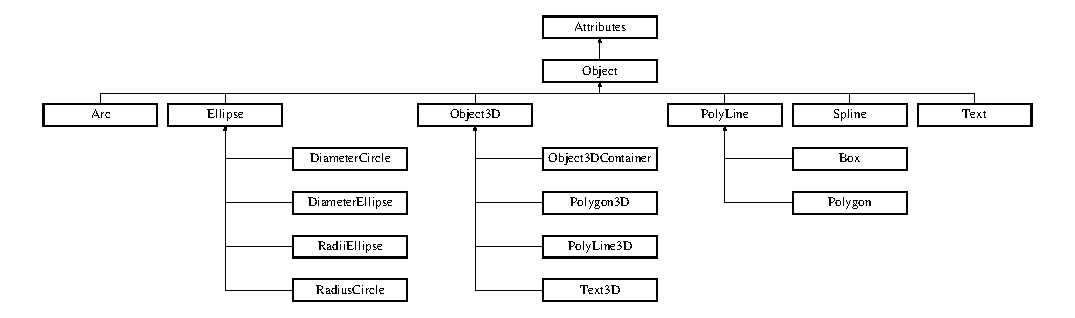
\includegraphics[height=3.82812cm]{classObject}
\end{center}
\end{figure}
\subsection*{Public Types}
\begin{CompactItemize}
\item 
enum {\bf Object\-Codes} \{ {\bf Pseudo\-Color\-Code} =  0, 
{\bf Arc\-Code} =  5, 
{\bf Compound\-Code} =  6, 
{\bf Ellipse\-Code} =  1, 
{\bf Poly\-Line\-Code} =  2, 
{\bf Spline\-Code} =  3, 
{\bf Text\-Code} =  4
 \}
\end{CompactItemize}
\subsection*{Public Methods}
\begin{CompactItemize}
\item 
{\bf Object} ()
\item 
virtual {\bf $\sim$Object} ()
\item 
{\bf Object\-Codes} {\bf get\-Code} ()
\item 
virtual void {\bf write} (std::ostream \&stream) const
\end{CompactItemize}
\subsection*{Protected Methods}
\begin{CompactItemize}
\item 
void {\bf set\-Code} ({\bf Object\-Codes} {\bf code})
\end{CompactItemize}
\subsection*{Protected Attributes}
\begin{CompactItemize}
\item 
{\bf Object\-Codes} {\bf code}
\end{CompactItemize}


\subsection{Detailed Description}
This generic class handles objects. This class is derived from {\bf Attributes} {\rm (p.\,\pageref{classAttributes})}. \begin{Desc}
\item[Author: ]\par
Anthony Liekens \end{Desc}




\subsection{Member Enumeration Documentation}
\index{Object@{Object}!ObjectCodes@{ObjectCodes}}
\index{ObjectCodes@{ObjectCodes}!Object@{Object}}
\subsubsection{\setlength{\rightskip}{0pt plus 5cm}enum Object::Object\-Codes}\label{classObject_s7}


Enumeration of object codes. The following object codes can be used to set the code of an object : \{$\backslash$tt Pseudo\-Color, {\bf Arc} {\rm (p.\,\pageref{classArc})}, Compound, Ellips, {\bf Poly\-Line} {\rm (p.\,\pageref{classPolyLine})}, {\bf Spline} {\rm (p.\,\pageref{classSpline})}, {\bf Text} {\rm (p.\,\pageref{classText})}\} \begin{Desc}
\item[Enumeration values: ]\par
\begin{description}
\index{PseudoColorCode@{PseudoColorCode}!Object@{Object}}\index{Object@{Object}!PseudoColorCode@{PseudoColorCode}}\item[{\em 
{\em Pseudo\-Color\-Code}\label{classObject_s7s0}
}]\index{ArcCode@{ArcCode}!Object@{Object}}\index{Object@{Object}!ArcCode@{ArcCode}}\item[{\em 
{\em Arc\-Code}\label{classObject_s7s1}
}]\index{CompoundCode@{CompoundCode}!Object@{Object}}\index{Object@{Object}!CompoundCode@{CompoundCode}}\item[{\em 
{\em Compound\-Code}\label{classObject_s7s2}
}]\index{EllipseCode@{EllipseCode}!Object@{Object}}\index{Object@{Object}!EllipseCode@{EllipseCode}}\item[{\em 
{\em Ellipse\-Code}\label{classObject_s7s3}
}]\index{PolyLineCode@{PolyLineCode}!Object@{Object}}\index{Object@{Object}!PolyLineCode@{PolyLineCode}}\item[{\em 
{\em Poly\-Line\-Code}\label{classObject_s7s4}
}]\index{SplineCode@{SplineCode}!Object@{Object}}\index{Object@{Object}!SplineCode@{SplineCode}}\item[{\em 
{\em Spline\-Code}\label{classObject_s7s5}
}]\index{TextCode@{TextCode}!Object@{Object}}\index{Object@{Object}!TextCode@{TextCode}}\item[{\em 
{\em Text\-Code}\label{classObject_s7s6}
}]\end{description}
\end{Desc}



\subsection{Constructor \& Destructor Documentation}
\index{Object@{Object}!Object@{Object}}
\index{Object@{Object}!Object@{Object}}
\subsubsection{\setlength{\rightskip}{0pt plus 5cm}Object::Object ()}\label{classObject_a0}


Constructor. This constructor does nothing special, since this is a generic and abstract class \index{Object@{Object}!~Object@{$\sim$Object}}
\index{~Object@{$\sim$Object}!Object@{Object}}
\subsubsection{\setlength{\rightskip}{0pt plus 5cm}Object::$\sim$Object ()\hspace{0.3cm}{\tt  [virtual]}}\label{classObject_a1}


Destructor. 

\subsection{Member Function Documentation}
\index{Object@{Object}!getCode@{getCode}}
\index{getCode@{getCode}!Object@{Object}}
\subsubsection{\setlength{\rightskip}{0pt plus 5cm}{\bf Object\-Codes} Object::get\-Code ()\hspace{0.3cm}{\tt  [inline]}}\label{classObject_a2}


Returns the code of an object \index{Object@{Object}!setCode@{setCode}}
\index{setCode@{setCode}!Object@{Object}}
\subsubsection{\setlength{\rightskip}{0pt plus 5cm}void Object::set\-Code ({\bf Object\-Codes} {\em code})\hspace{0.3cm}{\tt  [inline, protected]}}\label{classObject_b0}


Sets the code of an object. This method can only be called by instances of Object \begin{Desc}
\item[Parameters: ]\par
\begin{description}
\item[{\em 
code}]integer value \end{description}
\end{Desc}
\begin{Desc}
\item[Returns: ]\par
void \end{Desc}
\index{Object@{Object}!write@{write}}
\index{write@{write}!Object@{Object}}
\subsubsection{\setlength{\rightskip}{0pt plus 5cm}virtual void Object::write (std::ostream \& {\em stream}) const\hspace{0.3cm}{\tt  [inline, virtual]}}\label{classObject_a3}


Write the object to a given outstream. All inherited classes of object should provide this method, since it's called by {\bf Figure} {\rm (p.\,\pageref{classFigure})} (the object container) to output objects to a given stream. \begin{Desc}
\item[Parameters: ]\par
\begin{description}
\item[{\em 
stream}]output stream \end{description}
\end{Desc}
\begin{Desc}
\item[Returns: ]\par
void \end{Desc}


Reimplemented in {\bf Arc} {\rm (p.\,\pageref{classArc_a6})}, {\bf Ellipse} {\rm (p.\,\pageref{classEllipse_a13})}, {\bf Polygon3D} {\rm (p.\,\pageref{classPolygon3D_a8})}, {\bf Poly\-Line} {\rm (p.\,\pageref{classPolyLine_a4})}, {\bf Poly\-Line3D} {\rm (p.\,\pageref{classPolyLine3D_a8})}, {\bf Spline} {\rm (p.\,\pageref{classSpline_a5})}, {\bf Text} {\rm (p.\,\pageref{classText_a5})}, and {\bf Text3D} {\rm (p.\,\pageref{classText3D_a9})}.

\subsection{Member Data Documentation}
\index{Object@{Object}!code@{code}}
\index{code@{code}!Object@{Object}}
\subsubsection{\setlength{\rightskip}{0pt plus 5cm}{\bf Object\-Codes} Object::code\hspace{0.3cm}{\tt  [protected]}}\label{classObject_n0}




The documentation for this class was generated from the following files:\begin{CompactItemize}
\item 
{\bf object.h}\item 
{\bf object.cpp}\end{CompactItemize}
